\documentclass[11pt]{article}

%% LaTeX Preamble - Common packages

\usepackage[utf8]{inputenc}
\usepackage[spanish]{babel}
\usepackage{graphicx}
\usepackage{amsmath,amssymb}
\usepackage[left=2cm,right=2cm,top=2cm,bottom=2cm]{geometry}

\spanishdecimal{.}

\title{Primer examen parcial}
\author{Reconocimiento de Patrones (2024-2)}
\date{Julio Waissman Vilanova} 

%%% BEGIN DOCUMENT
\begin{document}

\maketitle

\vspace{5mm}

\textbf{Nombre}: \line(1,0){400}

\vspace{9mm}


\begin{enumerate}

\subsection*{Aprendizaje no supervisado}

\item ¿Qué ocurre si seleccionas un valor de $K$ demasiado alto en el algoritmo \emph{K--means}? ¿Cómo afecta esto a la segmentación de los datos y qué problemas podría generar en la interpretación de los resultados?

\vfill

\item ¿Qué sucede si eliges un valor de $\epsilon$ demasiado pequeño en el algoritmo DBSCAN? ¿Cómo afecta esto al número de clusters y a la cantidad de puntos clasificados como ruido?

\vfill

\item ¿Cuál es la importancia de estandarizar los datos antes de aplicar el Análisis de Componentes Principales, y qué podría suceder si omites este paso?

\vfill

\newpage

\subsection*{Aprendizaje PAC}

\item Consideremos el modelo de aprendizaje que vamos a llamar \emph{2--intervalos}. En este modelo $\mathcal{H}$ vamos a considerar que:
$$
h: \mathbb{R} \to \{-1, +1\},
$$
donde $h(x) = +1$ si el punto $x \in \mathbb{R}$ se encuentra dentro de alguno de dos intervalos (i.e. $[a, b]$ y $[c, d]$) preestablecidos. En caso contrario, $h(x) = -1$.

\vspace{3mm}

\begin{itemize}
    \item ¿Cual es el \emph{breakpoint} de $\mathcal{H}$?
    \vspace{3mm}
    \item ¿Que valor tiene $d_{VC}(\mathcal{H})$?
\end{itemize}

\vspace{3mm}

\item Ahora consideremos el caso genérico *$M$--intervalos*, donde $\mathcal{H}$ está definido como el conjunto de funciones $h: \mathbb{R} \to \{-1, +1\}$ tales que $h(x) = +1$ si $x$ se encuentra en alguno de los $M$ intervalos establecidos y $h(x) = -1$ en caso contrario.

\vspace{3mm}

\begin{itemize}
    \item ¿Que valor tiene $d_{VC}(\mathcal{H})$?
    \vspace{3mm}
    \item Si fueras a decidir utilizar un modelo $5$--intervalos, ¿Cuantos datos necesitarías como mínimo en tu conjunto de aprendizaje para asegurar la generalización?
\end{itemize}

\vspace{3mm}

\item Define con tus propias palabras que significa *Probablemente Aproximadamente Correcto (PAC)*

\newpage



\subsection*{Indicadores de desempeño}

\item Supongamos que tenemos un problema de inspección de piezas en una línea de producción. Se cuenta con un conjunto de datos de 1000 piezas, de las cuales 950 son piezas buenas y 50 son piezas defectuosas. Se utilizó un clasificador por regresión logística con una expansión polinomial de grado 2. Al generar la curva de aprendizaje obtenemos algo similar a la curva siguiente:

\begin{center}
  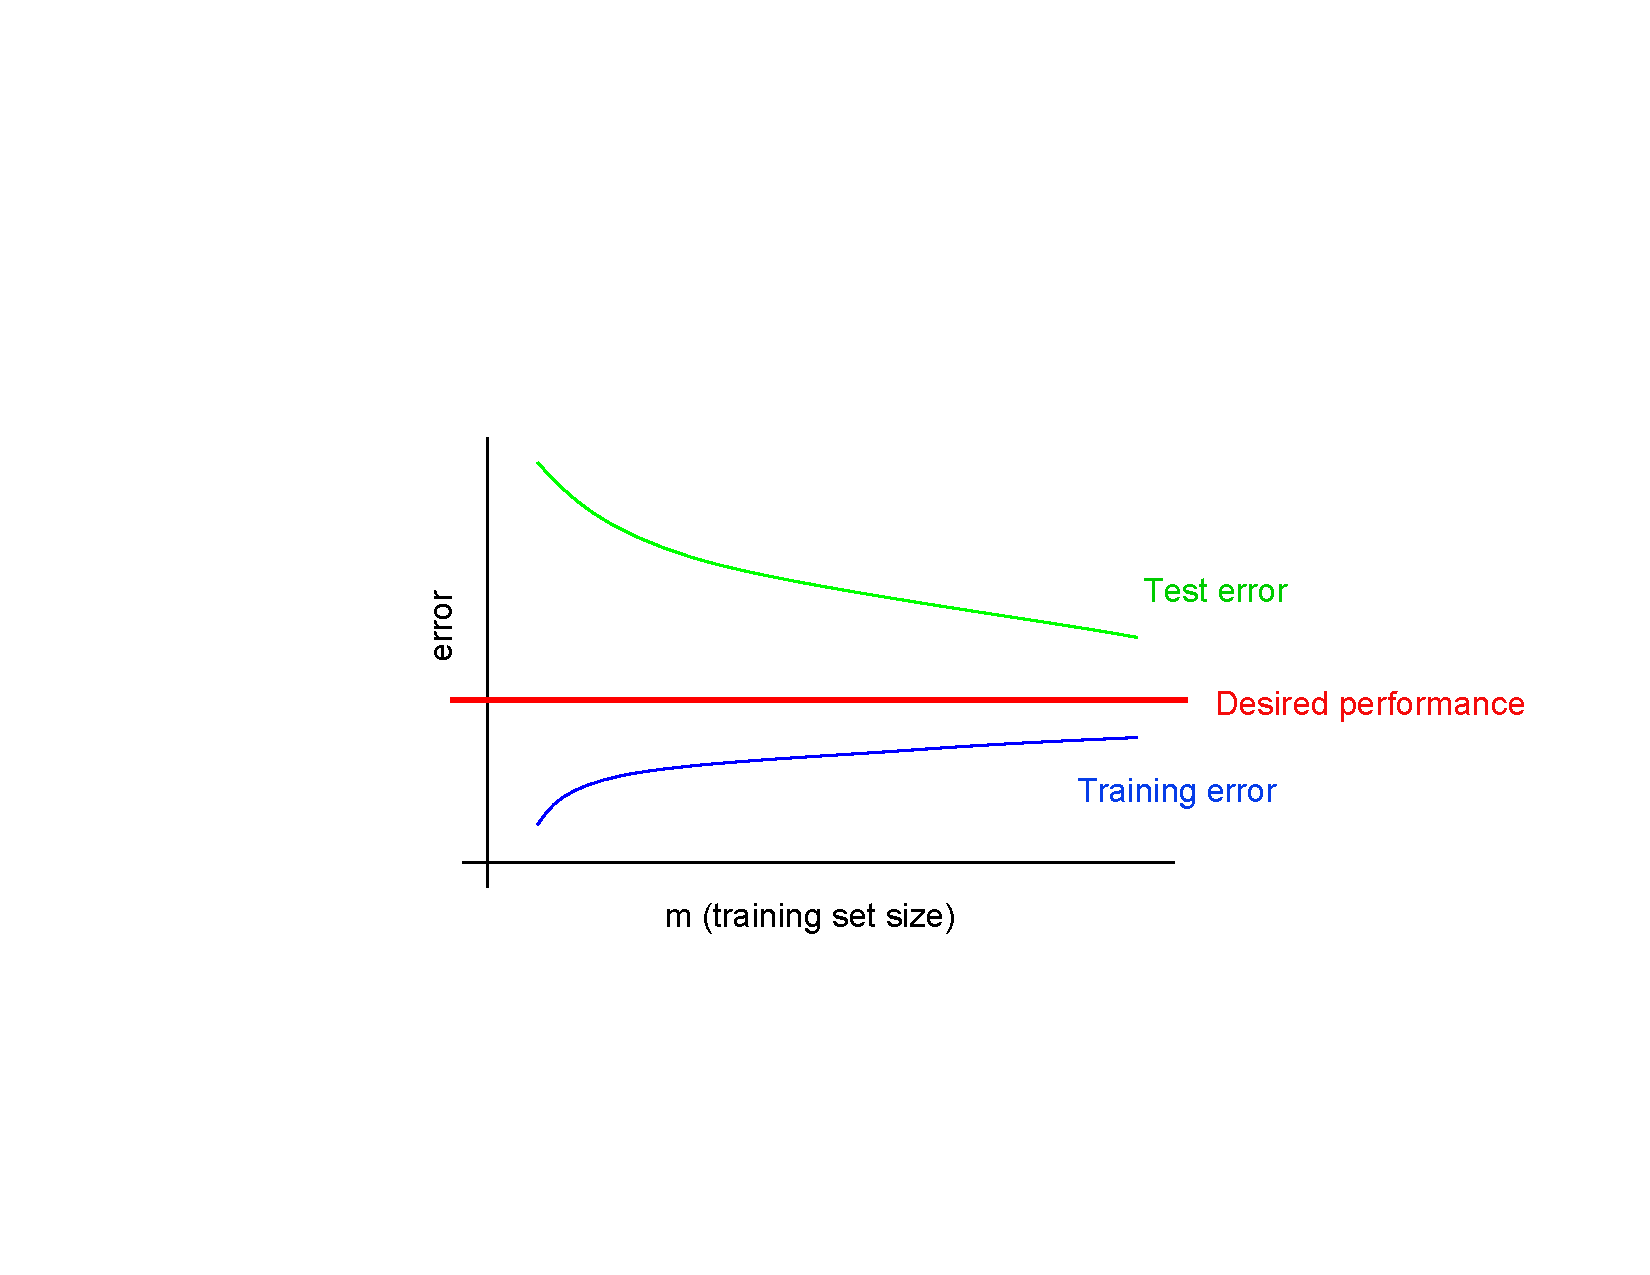
\includegraphics[width = 0.8\textwidth]{h_var.pdf}
\end{center}
subraya las acciones que podrían mejorar al modelo de aprendizaje.

\begin{itemize}
\item Solicitar la clasificación de más piezas.
\item Probar sin expansión polinomial.
\item Probar con una expansión polinomial de orden 3.
\item Usar PCA primero y quedarse con solo los componentes que expliquen el 95\% de la varianza.
\item Aumentar el valor de $\lambda$ (parámetro de regularización).
\item Disminuir el valor de $\lambda$ (parámetro de regularización).
\item Utilizar una SVM con kernel gaussiano.
\end{itemize}

\item Supongamos que estamos estimando la demanda de energia eléctrica doméstica
  en la Cd. de Hermosillo para el próximo día, utilizando como información el
  consumo de energía eléctrica de los 30 días anteriores, la temperatura máxima
  en Hermosillo de los 30 días anteriores, la temperatura mínima en Hermosillo
  de los 30 días anteriores, el día de la semana, una variable que indica si el
  día es festivo o no y una variable que indica la estación del año (invierno,
  primavera, verano y otoño). Se aplica un método de regresión lineal con la
  información de los últimos 5 años.

  Para analizar el desempeño del algoritmo de regresión lineal, se realiza una
  curva de aprendizaje la cual resulta ser de la forma siguiente:

  \begin{center}
    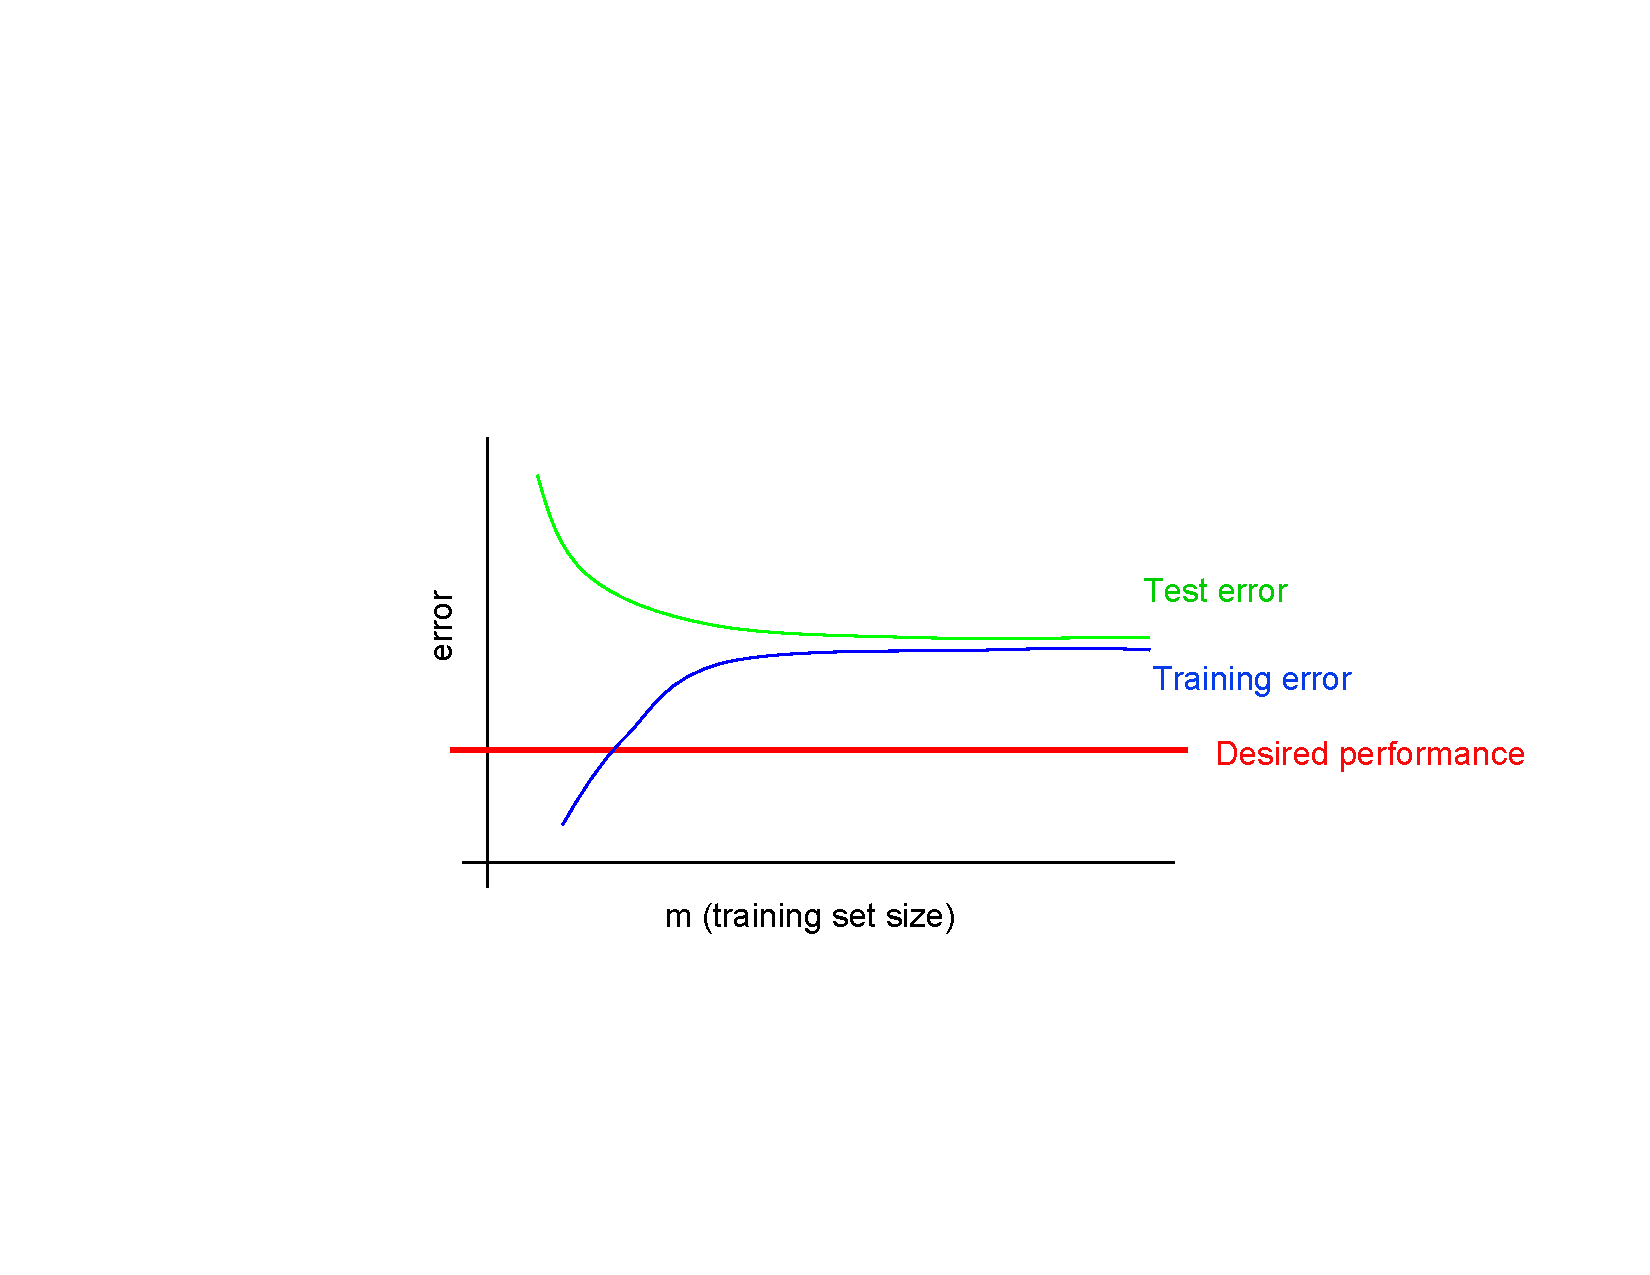
\includegraphics[width = 0.8\textwidth]{h_bia.pdf}
  \end{center}
  subraya las acciones que podrían mejorar al modelo de aprendizaje.

  \begin{itemize}
  \item Solicitarle a CFE información de otros 5 años anteriores.
  \item Disminuir el valor de $\lambda$ (parámetro de regularización).
  \item Aumentar el valor de $\lambda$ (parámetro de regularización).
  \item Utilizar solo la información histórica de los últimos 15 días y no de
    los 30 días anteriores.
  \item Utilizar una red neuronal en lugar de la regresión lineal.
  \item Agregar como atributos la raiz cuadrada de la demanda de energía
    eléctrica de los 30 días anteriores y la raiz cuadrada de los valores
    máximos y mínimos de temperatura de los 30 días anteriores.
  \item Agregar la humedad relativa de los 30 días anteriores.
  \end{itemize}

\item Sea la siguiente matriz de confusión, resuelta después de utilizar un
  método de aprendizaje para clasificar datos de un problema real:

  \begin{center}
    \begin{tabular}{cc}
      & $y$ \\
      $h_\theta(x)$ &
                      \begin{tabular}{c|cc}
                        & 0 & 1 \\
                        \hline
                        0 & 300 & 5 \\
                        1 & 10 & 30
                      \end{tabular}
    \end{tabular}
  \end{center}

  Responde a las siguientes preguntas:
  \vspace{3mm}
  \begin{enumerate}
  \item ¿Cual es el error de clasificación? 
  \vspace{3mm}
  \item ¿Cual es la precisión del clasificador? 
  \vspace{3mm}
  \item ¿Cual es el \emph{recall} del clasificador? 
  \vspace{3mm}
  \item ¿Cual es el $F_1$--score del clasificador? 
  \end{enumerate}


\end{enumerate}
\end{document}